\documentclass[aspectratio=169]{beamer}

\usepackage{tikz}
\usepackage{amsmath}
\usepackage{amssymb}

% ===== KCPC clean theme =====
\usetheme{default}
\useinnertheme{rectangles}
\useoutertheme{default}

\setbeamertemplate{navigation symbols}{}

% --- Colours ---
\definecolor{kcpc-bg}{RGB}{250,250,250}
\definecolor{kcpc-text}{RGB}{20,20,20}
\definecolor{kcpc-muted}{RGB}{90,90,90}
\definecolor{kcpc-red}{RGB}{176,0,0}

\setbeamercolor{background canvas}{bg=kcpc-bg}
\setbeamercolor{normal text}{fg=kcpc-text}
\setbeamercolor{frametitle}{fg=kcpc-text,bg=kcpc-bg}
\setbeamercolor{title}{fg=kcpc-text}
\setbeamercolor{subtitle}{fg=kcpc-muted}
\setbeamercolor{structure}{fg=kcpc-red}

\setbeamerfont{title}{series=\bfseries,size=\Large}
\setbeamerfont{frametitle}{series=\bfseries,size=\large}

\setlength{\parskip}{0.4em}

\setbeamertemplate{itemize item}{\(\rightarrow\)}
\setbeamertemplate{itemize subitem}{\(\rightarrow\)}

\setbeamertemplate{headline}{
    \vspace{0.2cm}
    \hspace{0.2cm}
    \textcolor{kcpc-muted}{\small\insertsection}
    \hfill
}

\setbeamertemplate{footline}{
    \hspace{0.2cm}
    \textcolor{kcpc-muted}{\small KCPC}
    \hfill
    \vspace{0.3cm}
}

\setbeamertemplate{background}{
    \begin{tikzpicture}[remember picture,overlay]
        \node[
            opacity=0.035,
            at=(current page.center)
        ] {
            % Replaced with a placeholder if the image isn't locally available during compilation
            
\includegraphics[width=0.55\paperwidth]{kcpc-logo.png}
        };
    \end{tikzpicture}
}

\AtBeginSection[]{
    \begin{frame}[plain]
        \vfill
        \centering
        {\Large\bfseries \insertsection}
        \vfill
    \end{frame}
}
% ============================

\title{Segment Trees in Competitive Programming}
\subtitle{Range Queries, Point Updates, and Laziness}
\author{KCPC Training}
\date{}

\begin{document}

\begin{frame}
    \titlepage
\end{frame}

\begin{frame}{Overview}
    \tableofcontents
\end{frame}

% ------------------------------------------------

\section{Module 0: Motivation}

\begin{frame}{The Core Problem}
    We begin with a very common task in competitive programming with \textit{queries}:

    Given an array \(a[0 \dots n-1]\), support:
    \begin{itemize}
        \item \textbf{Range sum query}
        $$
        \texttt{sum}(l,r) = \sum_{i=l}^{r} a[i]
        $$
        \item \textbf{Point update}
        $$
        \texttt{update}(pos,x): a[pos] = x
        $$
    \end{itemize}

    We want to answer many queries and updates efficiently, hopefully $10^5$ of them. So, it's a simple trade-off question:

    \begin{center}
        \textit{Can we make both operations fast at the same time?}
    \end{center}
\end{frame}

\begin{frame}{Naïve Approach}
    The simplest idea:
    \begin{itemize}
        \item For \(\texttt{sum}(l,r)\), loop from \(l\) to \(r\)
        \item For \(\texttt{update}(pos,x)\), just write \(a[pos] = x\)
    \end{itemize}

    \textbf{Complexity:}
    \begin{itemize}
        \item Query: \(\mathcal{O}(r-l+1)\), worst-case \(\mathcal{O}(n)\)
        \item Update: \(\mathcal{O}(1)\)
    \end{itemize}

    If we have \(q\) operations and many of them are long queries, total work becomes:
    $$
    \mathcal{O}(qn) \approx O(n^2) \text{ if } q \approx n
    $$

    Too slow for \(n, q \approx 10^5\).
\end{frame}

\begin{frame}{Prefix Sums}
    If the array were \textbf{static}, prefix sums would solve range sums perfectly. Define prefix sum as a cumulative array:
    $$
    pref[i] = a[0] + a[1] + \dots + a[i]
    $$

    Then:
    $$
    \texttt{sum}(l,r) =
    \begin{cases}
        pref[r] & l = 0 \\
        pref[r] - pref[l-1] & l > 0
    \end{cases}
    $$

    \begin{itemize}
        \item Query: \(\mathcal{O}(1)\)
        \item Update: \(\mathcal{O}(n)\), because all later prefix values change
    \end{itemize}

    So prefix sums are great for \textbf{read-only arrays}, but bad for
    \textbf{dynamic arrays}.
\end{frame}

\begin{frame}{The Trade-Off}
    So far we have two extremes:

    \begin{itemize}
        \item \textbf{Plain array}
        \begin{itemize}
            \item update fast
            \item query slow
        \end{itemize}
        \item \textbf{Prefix sums}
        \begin{itemize}
            \item query fast
            \item update slow
        \end{itemize}
    \end{itemize}

    What we really want is:
    \begin{itemize}
        \item logarithmic everything
        \item (or constant! but we won't have that today, unfortunately)
    \end{itemize}

    The key is to store answers as always but not just for prefixes, also for many intervals.
\end{frame}

% ------------------------------------------------

\section{Module 1: Segment Tree Intuition and Queries}

\begin{frame}{Main Intuition}
    Suppose we somehow knew:
    \begin{itemize}
        \item the sum of the whole array
        \item the sum of the left half and right half
        \item the sum of each quarter
        \item the sum of each eighth
        \item and so on...
    \end{itemize}

    Then many range queries could be answered by combining only a few precomputed pieces. Like how any natural number can be written in binary... This is exactly the \textbf{segment} tree's idea:
    \begin{itemize}
        \item each node corresponds to an interval
        \item each node stores the answer for that interval
        \item the interval is split into left half and right half
    \end{itemize}
\end{frame}

\begin{frame}{Tree of Intervals}
    \centering
    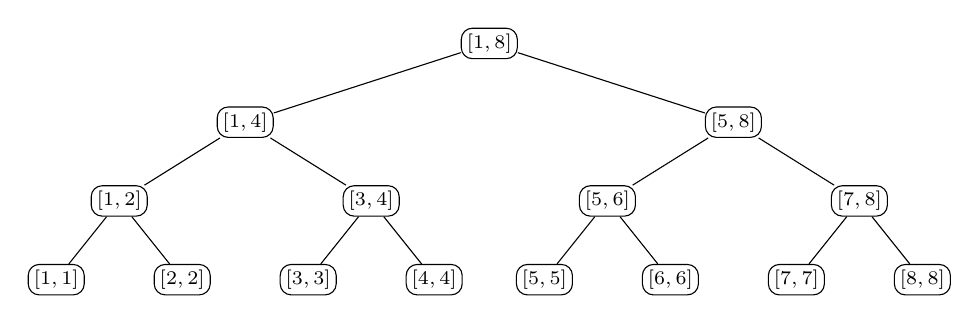
\begin{tikzpicture}[
        level distance=1.0cm,
        level 1/.style={sibling distance=6.2cm},
        level 2/.style={sibling distance=3.2cm},
        level 3/.style={sibling distance=1.6cm},
        every node/.style={
            draw,
            rounded corners,
            fill=white,
            inner sep=2pt,
            font=\scriptsize
        }
    ]
    \node {\([1,8]\)}
        child {
            node {\([1,4]\)}
            child {
                node {\([1,2]\)}
                child { node {\([1,1]\)} }
                child { node {\([2,2]\)} }
            }
            child {
                node {\([3,4]\)}
                child { node {\([3,3]\)} }
                child { node {\([4,4]\)} }
            }
        }
        child {
            node {\([5,8]\)}
            child {
                node {\([5,6]\)}
                child { node {\([5,5]\)} }
                child { node {\([6,6]\)} }
            }
            child {
                node {\([7,8]\)}
                child { node {\([7,7]\)} }
                child { node {\([8,8]\)} }
            }
        };
    \end{tikzpicture}

    \begin{itemize}
        \item The root represents the whole array.
        \item Leaves represent single elements.
        \item Internal nodes merge the answers of their children.
    \end{itemize}
\end{frame}

\begin{frame}{How a Query Uses the Tree}
    Suppose we want:
    $$
    \texttt{sum}(2,7)
    $$

    We may not have one node exactly equal to \([2,7]\), but we can decompose it into a
    few stored segments:
    $$
    [2,2] \cup [3,4] \cup [5,6] \cup [7,7]
    $$

    So:
    $$
    \texttt{sum}(2,7)
    =
    \texttt{val}([2,2])
    +
    \texttt{val}([3,4])
    +
    \texttt{val}([5,6])
    +
    \texttt{val}([7,7])
    $$

    The segment tree finds this \textbf{decomposition} quickly.
\end{frame}

\begin{frame}{Three Query Cases}
    Suppose a node covers \([tl,tr]\), and let
    $$
    tm = \left\lfloor \frac{tl+tr}{2} \right\rfloor
    $$

    For a query interval \([l,r]\), there are three possibilities:
    \begin{itemize}
        \item \textbf{Exact match:} \([l,r] = [tl,tr]\) \\
        Return the precomputed answer immediately.
        \item \textbf{Entirely in one child:} \\
        Recurse into left or right child only.
        \item \textbf{Intersects both children:} \\
        Split into two subqueries and merge the answers.
    \end{itemize}

    For sums, the merge operation is simply addition.
\end{frame}

\begin{frame}{Why is Query Time \(\mathcal{O}(\log n)\)?}
    The height of the tree is:
    $$
    \mathcal{O}(\log n)
    $$
    because the interval length is halved at every level.

    Also, a range query only branches near its two boundaries:
    \begin{itemize}
        \item one branch approaches the left boundary
        \item one branch approaches the right boundary
        \item fully covered middle segments stop immediately
    \end{itemize}

    So each level contributes only a constant number of useful nodes.

    Therefore:
    $$
    \texttt{query} = \mathcal{O}(\log n)
    $$
\end{frame}

\begin{frame}{How We Store the Tree}
    You could have some OOP practices with \texttt{Node} classes, but we are better than that: store the segment tree implicitly in an array of $t[4n]$.

    Convention:
    \begin{itemize}
        \item root at index \(1\)
        \item left child of \(v\) is \(2v\)
        \item right child of \(v\) is \(2v+1\)
    \end{itemize}

    The interval \([tl,tr]\) of a node is passed as function parameters.
\end{frame}

\begin{frame}[fragile]{Range Sum Query: Pseudocode}
\scriptsize
\begin{verbatim}
long long sum(int v, int tl, int tr, int l, int r) {
    if (l > r)
        return 0;

    if (l == tl && r == tr)
        return t[v];

    int tm = (tl + tr) / 2;

    return sum(v * 2, tl, tm, l, min(r, tm))
         + sum(v * 2 + 1, tm + 1, tr, max(l, tm + 1), r);
}
\end{verbatim}

    \normalsize
    \textbf{Idea:}
    \begin{itemize}
        \item if the current node exactly matches the query, use it
        \item otherwise ask only the necessary children
    \end{itemize}
\end{frame}

% ------------------------------------------------

\section{Module 2: Point Updates}

\begin{frame}{We Know How to Query --- But How Do We Update?}
    Suppose we perform:
    $$
    a[pos] = x
    $$

    Which nodes become invalid?
\end{frame}

\begin{frame}{Update Intuition}
    Only the nodes whose intervals contain \(pos\).

    That means:
    \begin{itemize}
        \item one leaf changes
        \item one node on each level lies on the path to that leaf
        \item all other nodes remain correct
    \end{itemize}

    So we only need to update a \textit{single root-to-leaf path}.

    Update strategy:
    \begin{enumerate}
        \item descend to the leaf representing \(a[pos]\)
        \item overwrite its value
        \item recompute every ancestor while returning upward
    \end{enumerate}

    So:
    $$
    \texttt{update} = \mathcal{O}(\log n)
    $$
\end{frame}

\begin{frame}[fragile]{Point Update: Pseudocode}
\scriptsize
\begin{verbatim}
void update(int v, int tl, int tr, int pos, int new_val) {
    if (tl == tr) {
        t[v] = new_val;
        return;
    }
    
    int tm = (tl + tr) / 2;

    if (pos <= tm)
        update(v * 2, tl, tm, pos, new_val);
    else
        update(v * 2 + 1, tm + 1, tr, pos, new_val);

    t[v] = t[v * 2] + t[v * 2 + 1];
}
\end{verbatim}

    \normalsize
    \begin{itemize}
        \item Leaf: directly store the new value.
        \item Internal node: recompute using the merge operation.
    \end{itemize}
\end{frame}

% ------------------------------------------------

\section{Module 3: Build}

\begin{frame}{Finally: How Do We Build the Tree?}
    So far, we assumed the tree already exists.

    To build it:
    \begin{itemize}
        \item each leaf gets its array value
        \item each internal node is merged from its two children
    \end{itemize}

    For a sum segment tree:
    $$
    t[v] = t[2v] + t[2v+1]
    $$

    This is naturally done with recursion.
\end{frame}

\begin{frame}{Build Intuition}
    Conceptually, build is bottom-up:
    \begin{itemize}
        \item leaves are known immediately
        \item parents are determined by children
        \item the root summarizes the whole array
    \end{itemize}

    In code we write it top-down:
    \begin{enumerate}
        \item build left child
        \item build right child
        \item merge them into the current node
    \end{enumerate}

    Each node is processed once, so:
    $$
    \texttt{build} = \mathcal{O}(n)
    $$
\end{frame}

\begin{frame}[fragile]{Build: Pseudocode}
\scriptsize
\begin{verbatim}
void build(vector<long long>& a, int v, int tl, int tr) {
    if (tl == tr) {
        t[v] = a[tl];
        return;
    }
    
    int tm = (tl + tr) / 2;

    build(a, v * 2, tl, tm);
    build(a, v * 2 + 1, tm + 1, tr);

    t[v] = t[v * 2] + t[v * 2 + 1];
}
\end{verbatim}

    \normalsize
    Main call:
    \begin{center}
        \texttt{build(a, 1, 0, n - 1);}
    \end{center}
\end{frame}

\begin{frame}{Basic Segment Tree Summary}
    \begin{center}
        \begin{tabular}{|l|c|c|}
        \hline
        \textbf{Method} & \textbf{Query} & \textbf{Update} \\
        \hline
        Naïve array & \(\mathcal{O}(n)\) & \(\mathcal{O}(1)\) \\
        \hline
        Prefix sums & \(\mathcal{O}(1)\) & \(\mathcal{O}(n)\) \\
        \hline
        Segment tree & \(\mathcal{O}(\log n)\) & \(\mathcal{O}(\log n)\) \\
        \hline
        \end{tabular}
    \end{center}

    Memory:
    $$
    \mathcal{O}(n)
    $$
    usually implemented as an array of size \(4n\). The same framework works for:
    \begin{itemize}
        \item sum
        \item minimum / maximum
        \item gcd
        \item counts
        \item and many, many more
    \end{itemize}
\end{frame}

% ------------------------------------------------

\section{Module 4: Let's be Lazy With this Problem}

\begin{frame}{Problem E: A Simple Task}
    We are given a string \(S\) of length \(n\), and \(q\) queries.

    Each query is:
    $$
    (l, r, k)
    $$
    meaning:
    \begin{itemize}
        \item if \(k = 1\), sort the substring \(S[l \dots r]\) in
        \textbf{non-decreasing} order
        \item if \(k = 0\), sort the substring \(S[l \dots r]\) in
        \textbf{non-increasing} order
    \end{itemize}

    Then output the final string after all queries.

    Constraints are large:
    \[
    n \le 10^5,\qquad q \le 5 \cdot 10^4
    \]

    So before we code anything, ask:
    \begin{center}
        \textit{What information do we really need in order to sort a
        substring?}
    \end{center}
\end{frame}

\begin{frame}{First Thought: Just Sort the Substring}
    A direct idea:
    \begin{itemize}
        \item extract \(S[l \dots r]\)
        \item sort it
        \item write it back
    \end{itemize}

    Or, since the alphabet is only lowercase English letters, use
    \textbf{counting sort}:
    \begin{itemize}
        \item count how many \texttt{a}, \texttt{b}, \dots, \texttt{z}
        are in the substring
        \item rewrite the substring in sorted order
    \end{itemize}

    For one query this costs: $\mathcal{O}(r-l+1 + 26)$

    In the worst case that becomes: $\mathcal{O}(nq)$, which is far too slow for \(10^5\)-scale input.
\end{frame}

\begin{frame}{A Better Way to Think About Sorting}
    Suppose we want to sort \(S[l \dots r]\) increasingly. We actually do \textbf{not} care about the old order inside the substring. We only care about the \textbf{frequency} of each character. So every query is really:
    \begin{enumerate}
        \item count how many times each character appears in \(S[l \dots r]\)
        \item rebuild the substring as blocks:
        \[
        \texttt{aaa}\dots\texttt{bbb}\dots\texttt{zzz}
        \]
        or the reverse order if \(k=0\)
    \end{enumerate}

    Example: $\texttt{cbaba} \xrightarrow{\text{sort increasing}} \texttt{aabbc}$

    So the real problem is no longer ``sorting''.
    It is:
    \begin{center}
        \textit{count letters on a range, then rewrite whole blocks quickly.}
    \end{center}
\end{frame}

\begin{frame}{What Operations Would Make This Easy?}
    For each character \(c \in \{\texttt{a}, \dots, \texttt{z}\}\),
    define a binary array:
    \[
    b_c[i] =
    \begin{cases}
        1 & \text{if } S[i] = c \\
        0 & \text{otherwise}
    \end{cases}
    \]

    Then for each character we would like to support:
    \begin{itemize}
        \item \textbf{Range sum query:} how many copies of \(c\) are in
        \([l,r]\)?
        \item \textbf{Range assignment:} set an entire interval to all \(0\)s
        or all \(1\)s
    \end{itemize}

    If we had these two operations, then sorting a substring would become
    straightforward.
\end{frame}

\begin{frame}{26 Segment Trees}
    This suggests the following structure:
    \begin{itemize}
        \item build \textbf{26 segment trees}
        \item tree \(c\) stores the binary array for character \(c\)
        \item node value = number of occurrences of that character in the
        segment
    \end{itemize}

    So for a query \([l,r]\):
    \begin{itemize}
        \item query all 26 trees to get the counts
        \item clear the whole interval \([l,r]\)
        \item write back character blocks in increasing or decreasing order
    \end{itemize}

    This is a \textit{beautiful} plan.

    But there is one missing ingredient:
    \begin{center}
        \textbf{how do we update a whole range quickly?}
    \end{center}
\end{frame}

\begin{frame}{Okay --- If We Had This Range Update, We Would Be Done}
    In one character tree, we need:
    \begin{itemize}
        \item \(\texttt{sum}(l,r)\): count 1s in a range
        \item \(\texttt{assign}(l,r,0)\): erase a block
        \item \(\texttt{assign}(l,r,1)\): fill a block
    \end{itemize}

    A normal segment tree already gives us fast range sums.

    The problem is the assignment.
    If we assign position by position, then rewriting a long substring is
    expensive again.

    So the next question is:
    \begin{center}
        \textit{Can we delay work, but still keep the answers correct? Can we be \textbf{lazy}?}
    \end{center}
\end{frame}

\begin{frame}{Lazy Propagation Intuition}
    Suppose a node covers the interval \([tl,tr]\), and we learn that
    \textbf{every value in this whole interval becomes \(0\)}.

    Do we really need to immediately visit every child and every leaf?

    \pause

    \textbf{No.}

    Instead, we can:
    \begin{itemize}
        \item immediately fix the answer for the current node
        \item store a small note saying:
        \begin{center}
            \textit{``if anyone later asks about my children,
            remember that they should all become \(0\)''}
        \end{center}
        \item only push that information downward when it becomes necessary
    \end{itemize}

    This is exactly the idea of \textbf{lazy propagation}:
    \begin{center}
        \textit{postpone detailed updates until they are actually needed}
    \end{center}
\end{frame}

\begin{frame}{What a Node Stores in One Character Tree}
    For one fixed character:
    \begin{itemize}
        \item \(t[v]\) = how many 1s are in this segment
        \item \(\texttt{lazy}[v]\) stores a pending assignment
    \end{itemize}

    For the lazy tag we use:
    \begin{itemize}
        \item \(-1\): no pending update
        \item \(0\): this whole segment should be all zeros
        \item \(1\): this whole segment should be all ones
    \end{itemize}

    If a segment \([tl,tr]\) is entirely assigned to \(x \in \{0,1\}\), then:
    \[
    t[v] = (tr - tl + 1)\cdot x
    \]

    That is enough to answer sums on this whole segment immediately,
    without touching the children yet.
\end{frame}

\begin{frame}[fragile]{Lazy Propagation: \texttt{apply} and \texttt{push}}
\scriptsize
\begin{verbatim}
void apply(int v, int tl, int tr, int val) {
    t[v] = (tr - tl + 1) * val;
    lazy[v] = val;   // val is 0 or 1
}

void push(int v, int tl, int tr) {
    if (lazy[v] == -1 || tl == tr) return;
    int tm = (tl + tr) / 2;
    apply(v * 2, tl, tm, lazy[v]);
    apply(v * 2 + 1, tm + 1, tr, lazy[v])
    lazy[v] = -1;
}
\end{verbatim}

    \normalsize
    \begin{itemize}
        \item \texttt{apply} updates the current segment immediately
        \item \texttt{push} forwards postponed information to the children
        \item we only push when we need to go deeper
    \end{itemize}
\end{frame}

\begin{frame}[fragile]{Range Assign}
\scriptsize
\begin{verbatim}
void assign(int v, int tl, int tr, int l, int r, int val) {
    if (l > r)
        return;
    if (l == tl && r == tr) {
        apply(v, tl, tr, val);
        return;
    }

    push(v, tl, tr);
    int tm = (tl + tr) / 2;

    assign(v * 2, tl, tm, l, min(r, tm), val);
    assign(v * 2 + 1, tm + 1, tr, max(l, tm + 1), r, val);

    t[v] = t[v * 2] + t[v * 2 + 1];
}
\end{verbatim}
\end{frame}

\begin{frame}[fragile]{Range Sum}
\scriptsize
\begin{verbatim}
int sum(int v, int tl, int tr, int l, int r) {
    if (l > r)
        return 0;
    if (l == tl && r == tr)
        return t[v];

    push(v, tl, tr);
    int tm = (tl + tr) / 2;

    return sum(v * 2, tl, tm, l, min(r, tm))
         + sum(v * 2 + 1, tm + 1, tr, max(l, tm + 1), r);
}
\end{verbatim}
\end{frame}

\begin{frame}{How One Query is Processed}
    Now the whole problem becomes systematic.

    For a query \((l,r,k)\):
    \begin{enumerate}
        \item For each character \(c\), compute
        \(\texttt{cnt}[c] = \texttt{sum}_c(l,r)\)
        \item For each character tree, assign \([l,r]\) to \(0\)
        \item Rebuild the segment using blocks of characters:
        \begin{itemize}
            \item if \(k=1\): from \(\texttt{a}\) to \(\texttt{z}\)
            \item if \(k=0\): from \(\texttt{z}\) to \(\texttt{a}\)
        \end{itemize}
        \item If \(\texttt{cnt}[c] = x\), assign the next block of length
        \(x\) to \(1\) in tree \(c\)
    \end{enumerate}

    So the substring is rebuilt in sorted order using only
    \textbf{range sums + range assignments}.
\end{frame}

\begin{frame}[fragile]{High-Level Query Routine}
\scriptsize
\begin{verbatim}
for (int c = 0; c < 26; c++) {
    cnt[c] = tree[c].sum(1, 1, n, l, r);
    tree[c].assign(1, 1, n, l, r, 0);
}

int cur = l;

if (k == 1) for (int c = 0; c < 26; c++) {
    if (cnt[c] == 0) continue;
    tree[c].assign(1, 1, n, cur, cur + cnt[c] - 1, 1);
    cur += cnt[c];
} else for (int c = 25; c >= 0; c--) {
    if (cnt[c] == 0) continue;
    tree[c].assign(1, 1, n, cur, cur + cnt[c] - 1, 1);
    cur += cnt[c];
}
\end{verbatim}
\end{frame}

\begin{frame}{Why This Works}
    The correctness is driven by two simple facts:

    \begin{itemize}
        \item Querying all 26 trees gives the exact number of each character
        in the substring.
        \item After clearing \([l,r]\), we place back exactly the same total
        number of characters, only in a new order.
    \end{itemize}

    Therefore:
    \begin{itemize}
        \item the \textbf{multiset} of letters in the substring is preserved
        \item writing blocks from \(\texttt{a}\) to \(\texttt{z}\) gives
        non-decreasing order
        \item writing blocks from \(\texttt{z}\) to \(\texttt{a}\) gives
        non-increasing order
    \end{itemize}

    So every query performs exactly the required sort.
\end{frame}

\begin{frame}{Complexity}
    For each query:
    \begin{itemize}
        \item 26 range-sum queries to count characters
        \item 26 range assignments to clear the interval
        \item up to 26 range assignments to rebuild it
    \end{itemize}

    Each operation costs: $\mathcal{O}(\log n)$

    So one query costs: $\mathcal{O}(26 \log n)$

    Since the alphabet size is constant, this is effectively: $\mathcal{O}(\log n)\ \text{per query}$

    Overall: $\mathcal{O}(q \cdot 26 \log n)$, which is fast enough.
\end{frame}

\begin{frame}{Takeaway: Segment Tree: Very Powerful TOOL}
    \begin{itemize}
        \item Segment tree is a very important thing in competitive programming.
        \item There are very weird ways to use it: multi-dimensional segment trees, segment tree beats, persistent segment tree, dynamic segment tree, ...
        \item You can have generalised segment tree implementations. Look at AtCoder Library for an abstract template.
        \item Though, never have The Grudge against segment tree.
    \end{itemize}
\end{frame}

% ------------------------------------------------

% \begin{frame}[plain]
%     \vfill
%     \centering
%     {\Large\bfseries Problem solving}

%     \vspace{0.5cm}
%     \textcolor{kcpc-muted}{Now let's implement and use it.}
%     \vfill
% \end{frame}

\end{document}